\documentclass[12pt,oneside,english]{article}

\usepackage[T1]{fontenc}
\usepackage[latin1]{inputenc}
\usepackage{geometry}
\geometry{verbose,letterpaper,tmargin=1in,bmargin=1in,lmargin=1in,rmargin=1in}
\usepackage{textcomp}
\usepackage{babel}
\setcounter{secnumdepth}{0}
\usepackage{graphicx}
\usepackage{float}
\floatstyle{boxed}
\restylefloat{figure}
\usepackage{longtable}
\usepackage{url}

\usepackage{courier}
\usepackage{color}
\usepackage{listings}

\definecolor{dkgreen}{rgb}{0,0.6,0}
\definecolor{gray}{rgb}{0.5,0.5,0.5}

\newbox\bwk\edef\tempd#1pt{#1\string p\string t}\tempd\def\nbextr#1pt{#1}
\def\npts#1{\expandafter\nbextr\the#1\space}
\def\ttwplink#1#2{\special{ps:1 0 0 setrgbcolor}#2\special{ps:0 0 0 setrgbcolor}\setbox\bwk=\hbox{#2}\special{ps:( linkto #1)\space\npts{\wd\bwk} \npts{\dp\bwk} -\npts{\ht\bwk} true\space Cpos}}


\begin{document}

	\title{Grain Size Analysis}
	
	\maketitle

	\begin{figure}
	\center
	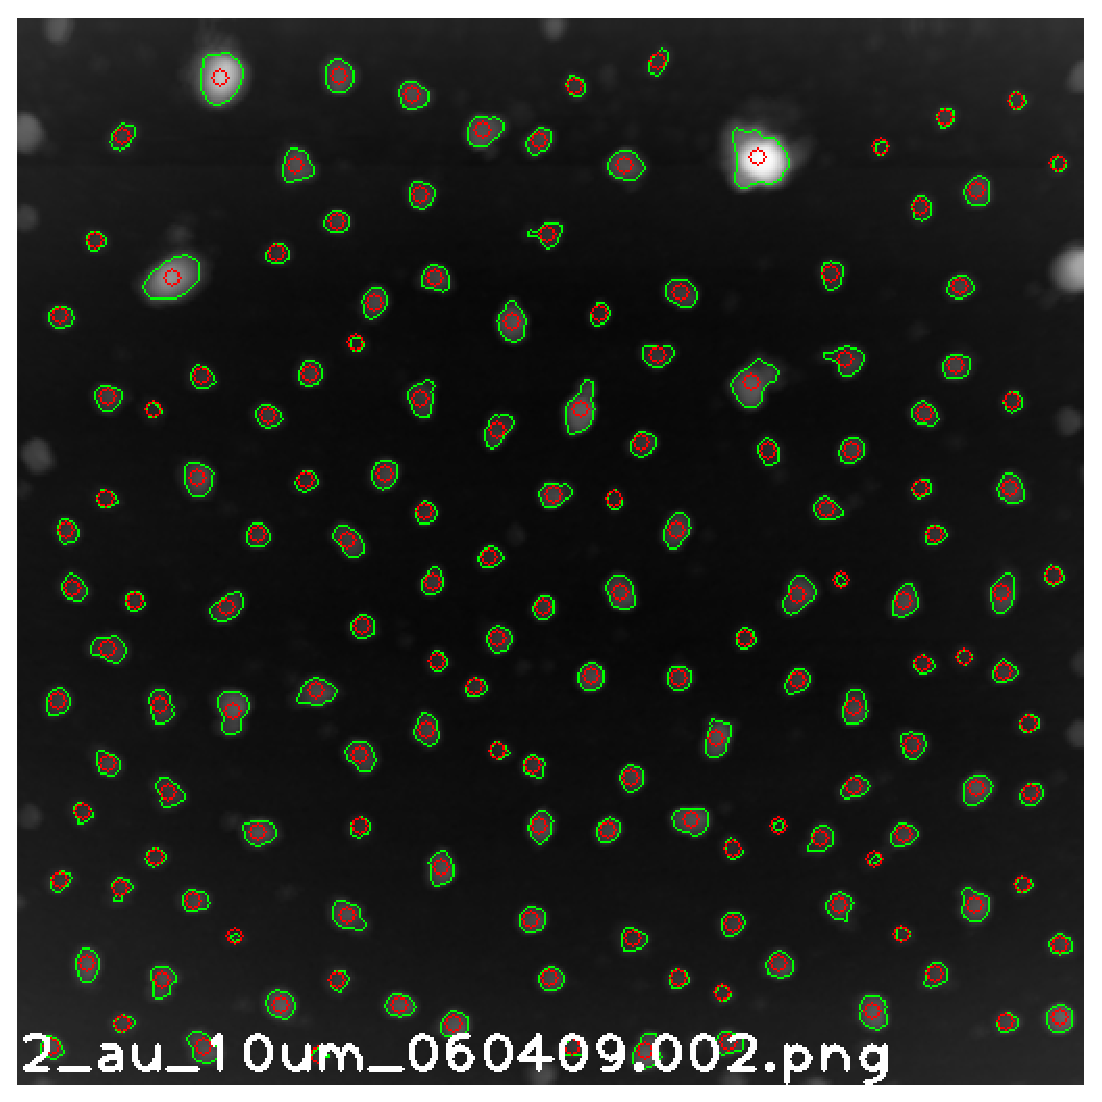
\includegraphics[width=100mm]{images/2_au_10um_060409.002.png_adt71_flr8_minsz10_outlines.eps}
	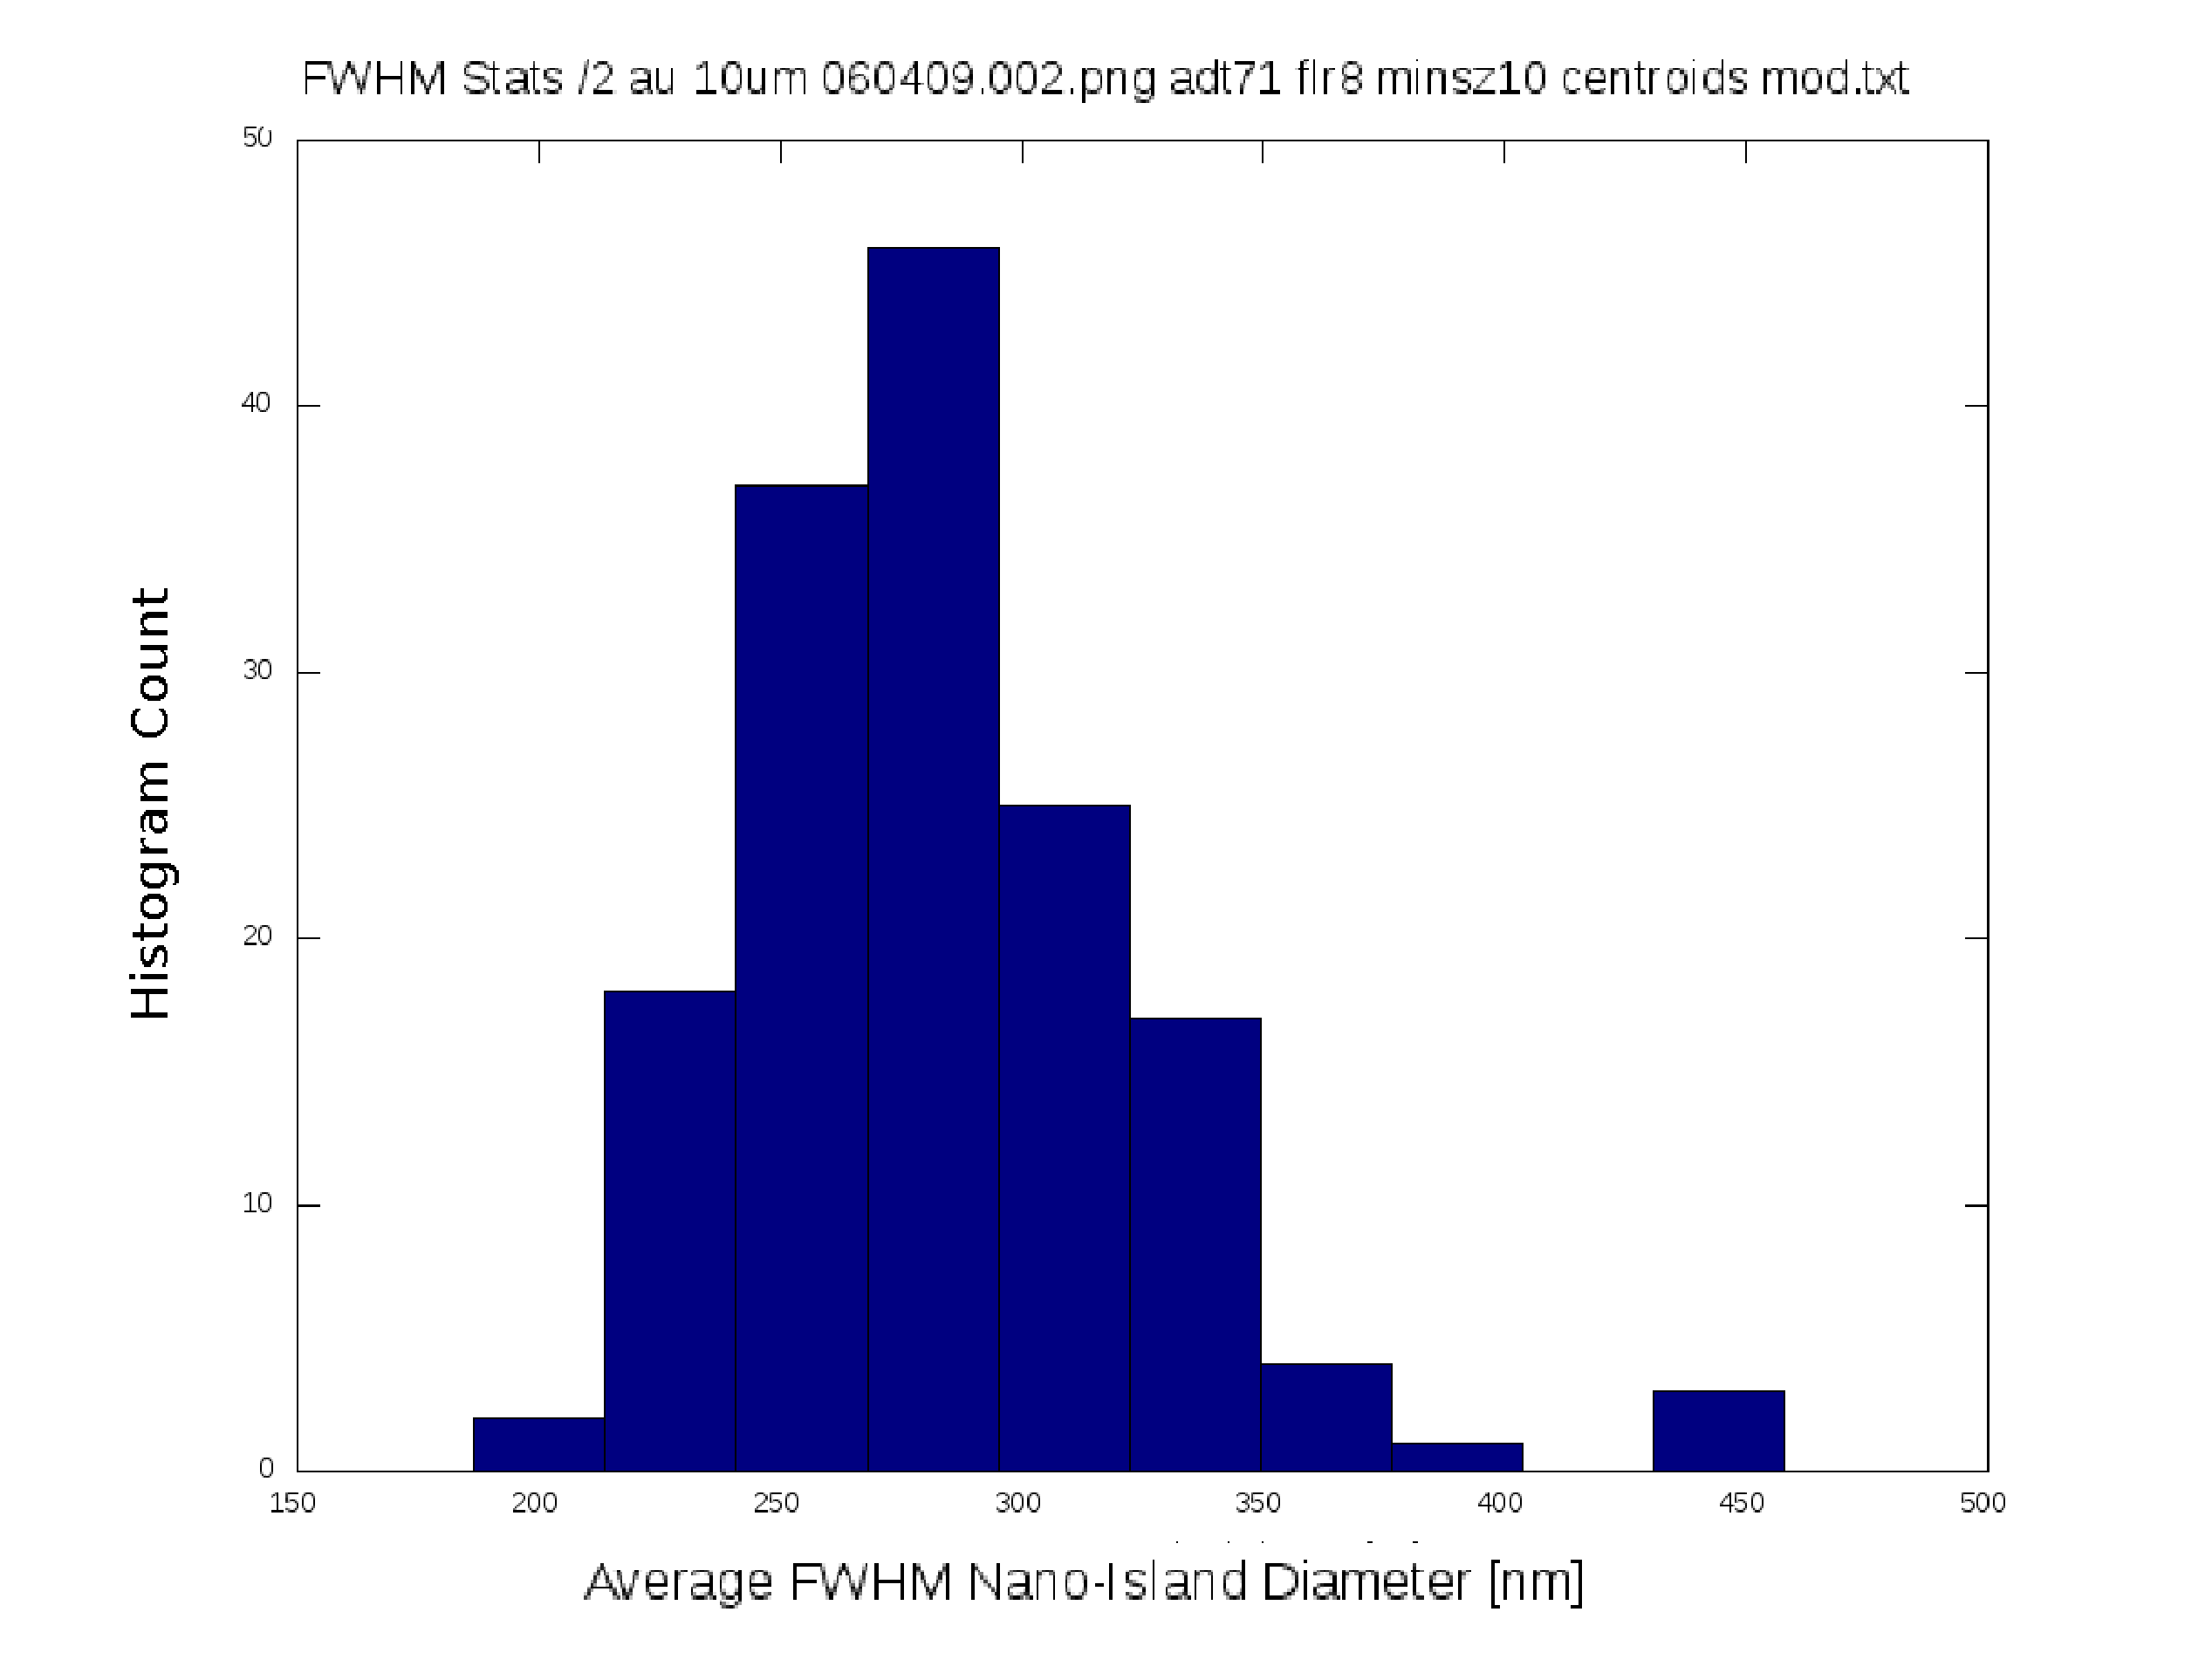
\includegraphics[width=140mm]{images/2_au_10um_060409.002.png_adt71_flr8_minsz10_histogram_fwhm.eps}
	\caption{Computer Vision Result}
	\label{f:cvPromo}
	\end{figure}

	[Figure 1 should show the result of automated analysis -- first image illustrates the automated grain size analysis result]

	Use of computer vision libraries is proposed to calculate the cross-sectional area of gold nano-islands formed by the self-assembly process.  
		
	This section defines a software approach that applies computer vision to partially automate the measurement of island size.


	\section{A comparison of methods for calculating size in self-assebled gold nano-islands}
	% This section presents the teaser -- a default watershed takes time to configure with weird result

	\begin{figure}
	\center
	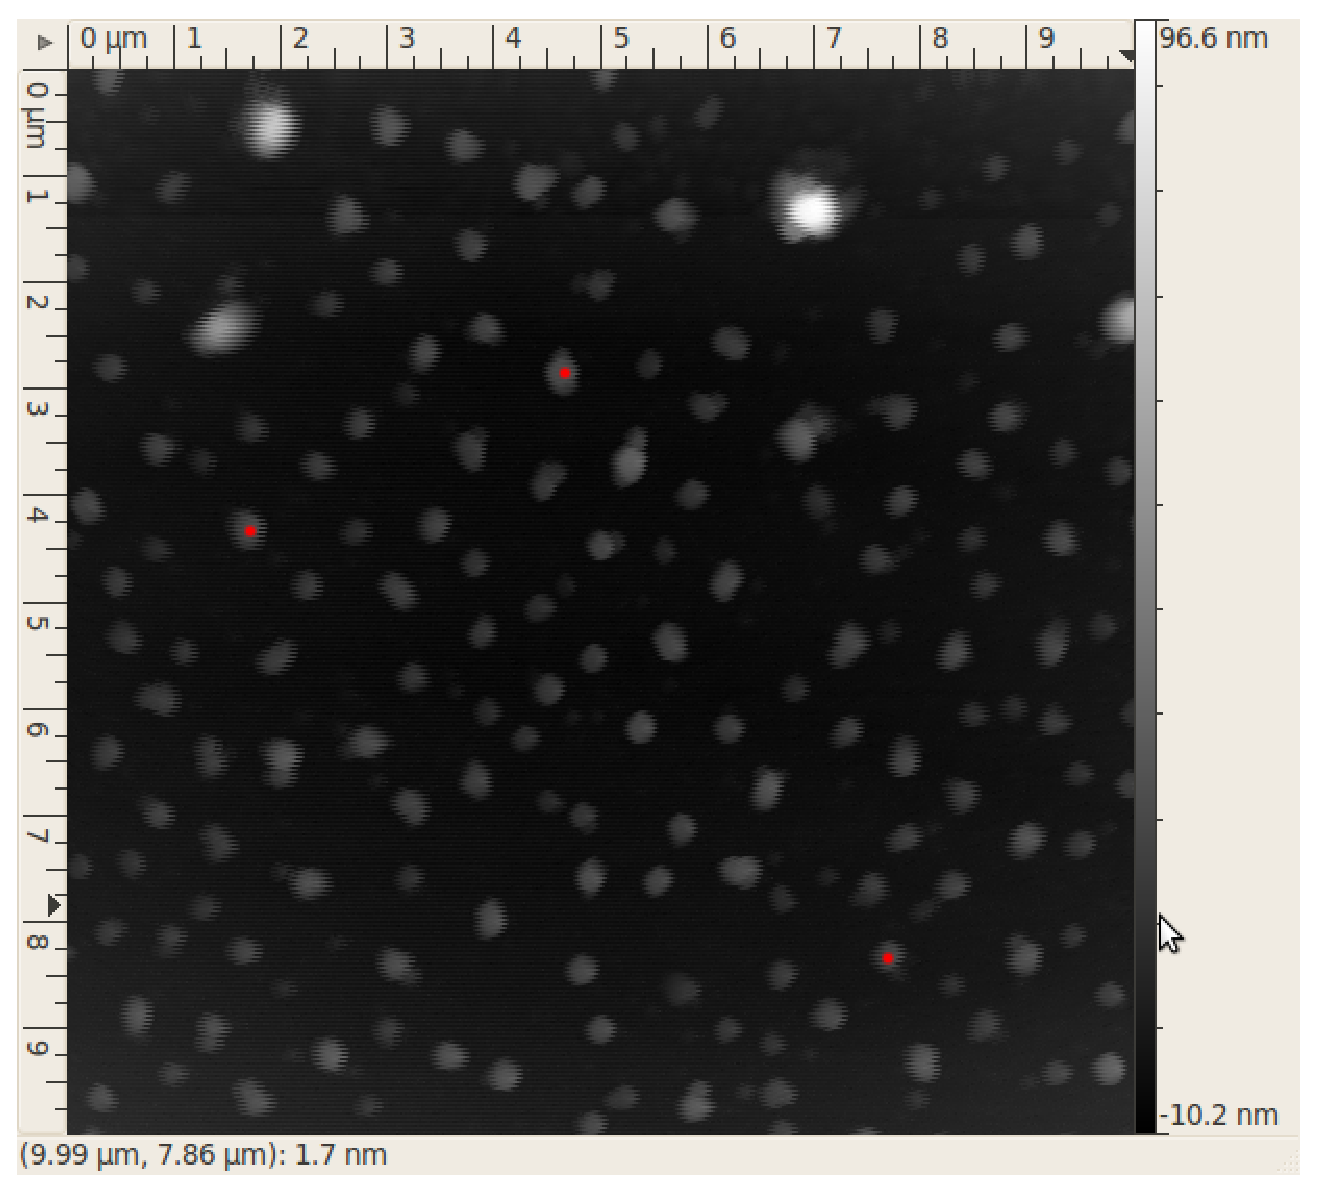
\includegraphics[width=140mm]{images/gwyddion-original-spots.eps}
	\caption{Isolated nano-islands separated by large gaps challenge the watershed method for determining the size of each island.  Visually, we can see that the islands (such as the three islands identified by red dots) are a quarter-micron in diameter, but a poorly-tuned watershed method easily underestimates the island size.}
	\label{f:gwyOrig}
	\end{figure}
	
	Nano-island measurements analyzed with a default AFM image watershed in Gwyddion disagreed with image cross-sections.  
	This problem motivated development of a computer vision approach to automate an alternate process to the default watershed.

	\subsection{A test of the watershed method versus cross-section FWHM}
	
		For isolated nano-islands of material separated by a ``no man's land'' of a blank substrate (as in Figure \ref{f:gwyOrig}), the extent of the islands can be visually approximated by an analyst.
		The island is easily interpreted by a human observer as a bright spot on a dark background, and the size is checked against the rulers along the horizontal and vertical image axes. 
			
		A better size estimate for an eliptical island would use image cross-sections across major and minor axes to determine how far the island rises above the background.
		A metric such as Full-Width at Half-Maximum (FWHM) can be used to estimate the extent of the major and minor axis for eliptical islands.
			
%	A full analysis of island size would require a histogram of island sizes to be measured.  
%	A histogram using this method would require the analyst to draw one or more cross-sections (such as along the major and minor axes) across each of the islands in the image, for all images in the measurement set.
	
	\subsubsection{Analysis of a sample image by manually-selected cross-sections}
		  
		In this section, islands are found visually and measured manually. 
	For a comparison with the watershed method, cross-sections were drawn across six representative islands to produce size estimates as would be calculated by a human analyst.  
	Each cross-section produces a data set with values for distance (along the cross-section line) and height for the island cross-section.  
	Cross-section data was exported from a Gwyddion data set to a text file, then converted to Matlab-readable array (Listing \ref{lst:Xdata}).   
	
	The FWHM for each trace was calculated by the GNU Octave ``fwhm'' function as follows (Listing \ref{lst:Fwhm}).

\lstset{language=Matlab,
   keywords={break,case,catch,continue,else,elseif,end,for,function,
      global,if,otherwise,persistent,return,switch,try,while},
   basicstyle=\sffamily,
   keywordstyle=\color{blue},
   commentstyle=\color{dkgreen},
   stringstyle=\color{red},
   numbers=left,
   numberstyle=\tiny\color{gray},
   stepnumber=1,
   backgroundcolor=\color{white},
   tabsize=4,
   showspaces=false,
   showstringspaces=false}

\lstset{caption=function wraps Gwyddion cross-section data, label=lst:Xdata}
\lstinputlisting{./codedir/cross_section_sample.m}


\lstset{caption=function to calculate FWHM from data, label=lst:Fwhm}
\lstinputlisting{./codedir/do_fwhm.m}


	\begin{figure}
	\center
	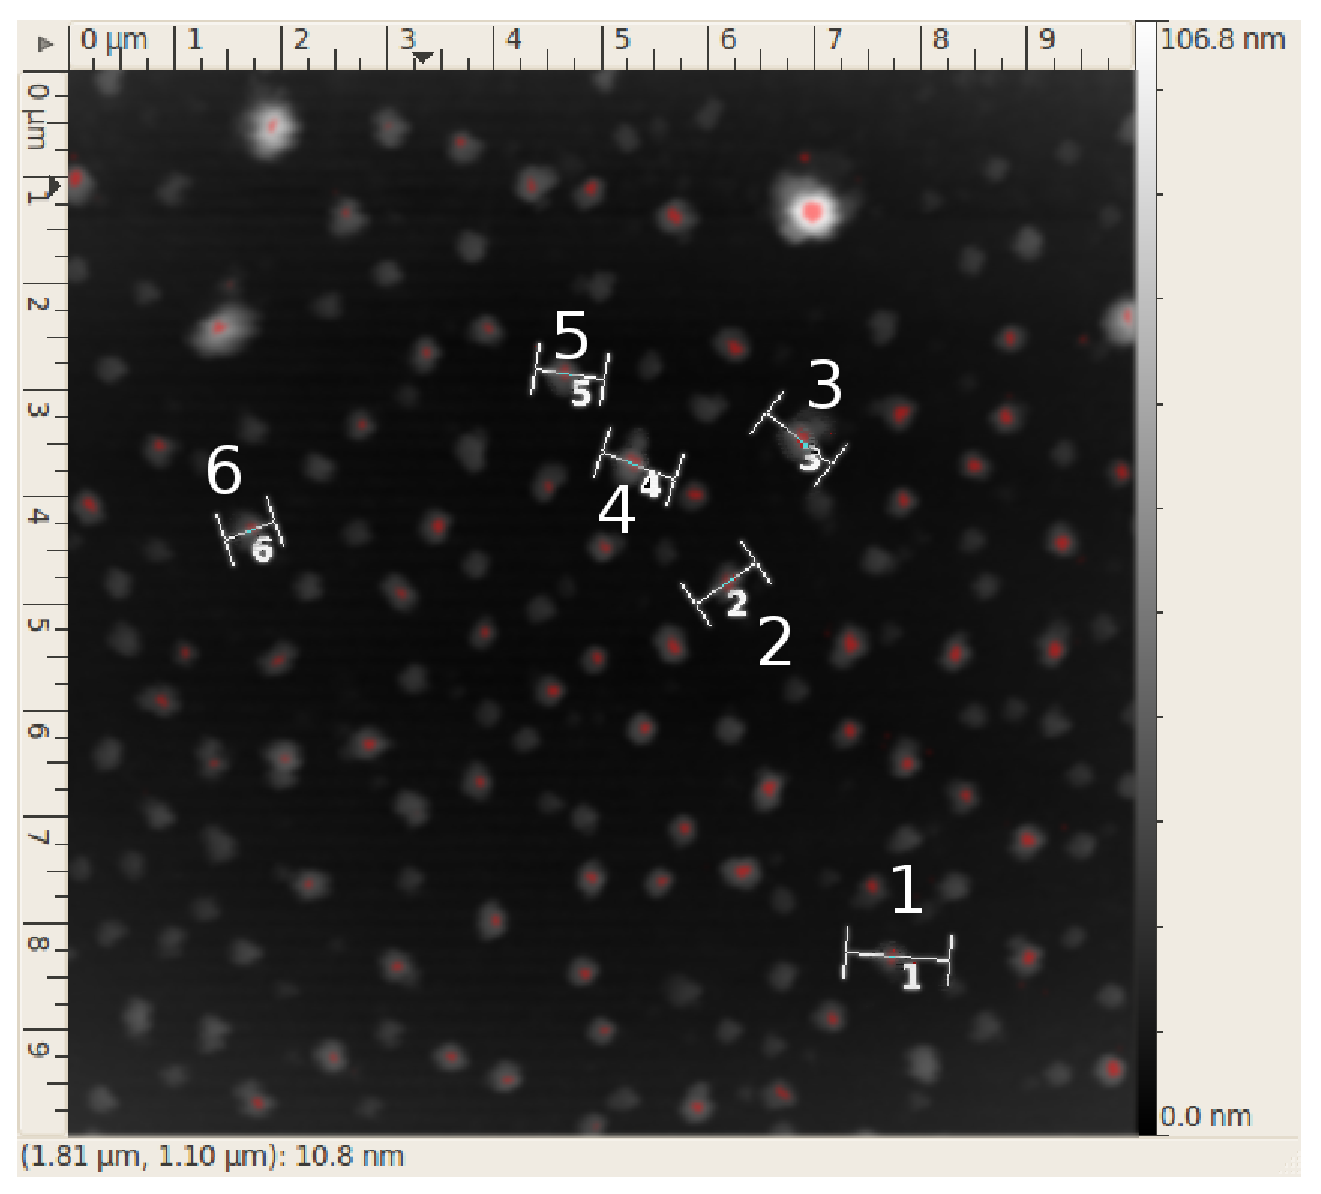
\includegraphics[width=140mm]{images/gwyddion-cross-sections.eps} 
	\caption{A watershed grain analysis was run using default parameters in Gwyddion (reference).  Several cross-sections were also selected, and full-width at half maximum was calculated for each.  The watershed grains were of mean diameter $90nm$ (Figure \ref{f:gwyXcurves}).  The cross-section FWHM for the six islands labeled above were calculated as $1: 216nm , 2: 286nm , 3: 304nm , 4: 229nm , 5: 233nm , 6: 241nm$, which match an analyst's estimate of a quarter-micron island size.}
	\end{figure}
		
	\begin{figure}
	\center
	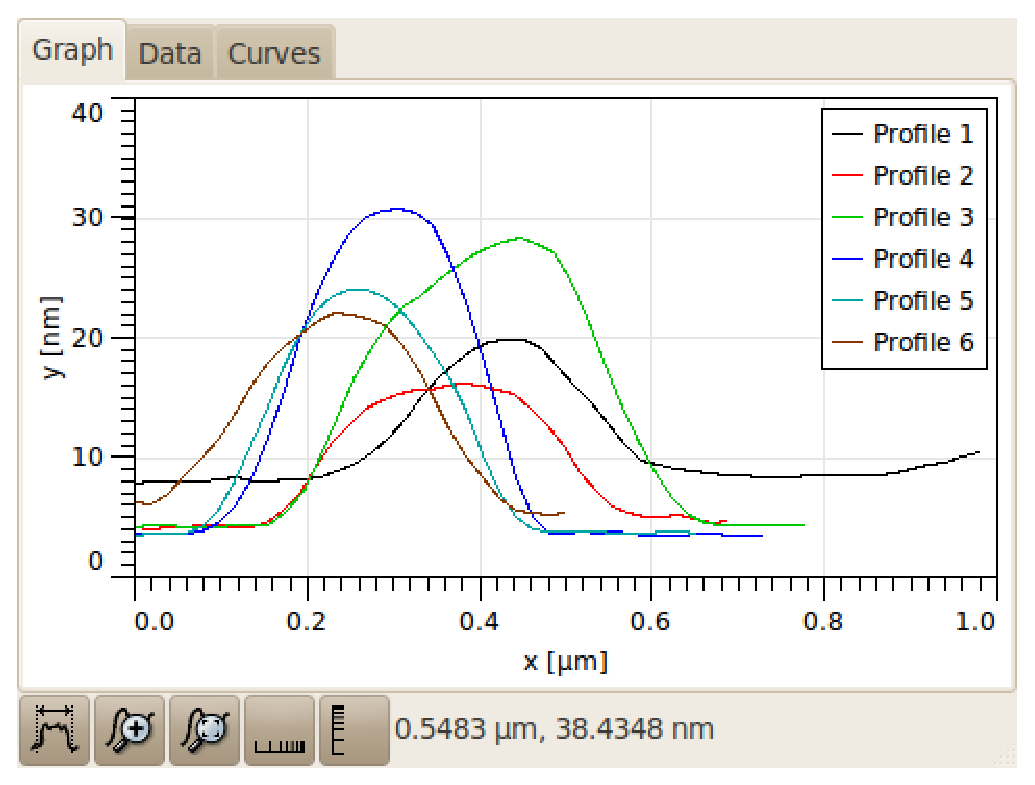
\includegraphics[width=140mm]{images/gwyddion-cross-section-curves.eps}
	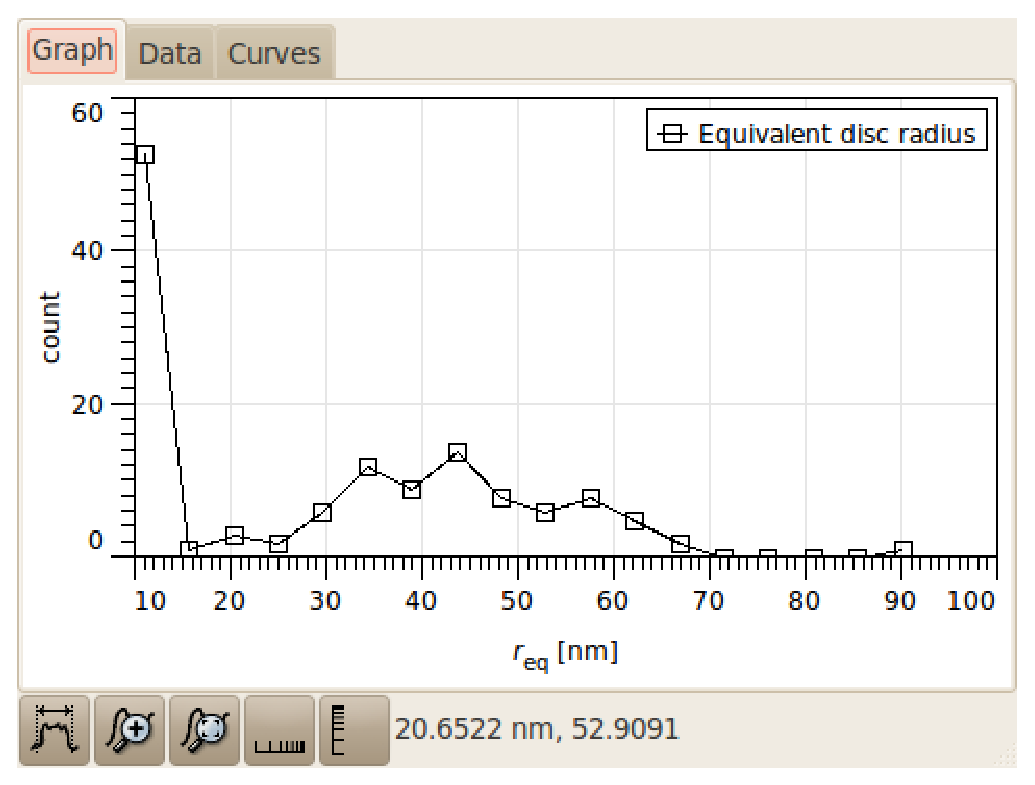
\includegraphics[width=140mm]{images/gwyddion-watershed-radius.eps}
	\caption{The watershed produced a grain size that does not agree with the FWHM samples.  Although the disk radius is visually and graphically a quarter-micron in diameter (top), the default Gwyddion watershed produces a distribution with an average of 90 microns diameter (bottom).  The top plot shows cross-sections for six grains, and the bottom plot shows the ``equivalent disk radius'' watershed result.1}\\
	\label{f:gwyXcurves}
	\end{figure}



	\section{Grain Size Analysis Through Computer Vision}
	
	\subsection{Introduction: The Gwyddion watershed}
	% The 

	The watershed method is ideally suited for calculating grain size in cross-sections of metal, crystalline materials, or contiguous thin films [minimum spanning forests paper].  
	In the case of nano-islands, the ``grains'' consist  of mostly-isolated lumps of gold which can be separated by a zone that should not belong to any watershed.
	
	[``Watershed Cuts: Minimum Spanning Forests and the Drop of Water Principle'' by 
	Jean Cousty, Gilles Bertrand, Laurent Najman, and Michel Couprie
	
	IEEE TRANSACTIONS ON PATTERN ANALYSIS AND MACHINE INTELLIGENCE, VOL. 31, NO. 8, AUGUST 2009]

	Past analysis of nano-island size overcame watershed limitations with student labor (conversation, Chuhee Kwon, 2013-08-28, 10:15am).  
	Watershed parameters were tuned to a particular image, and grains were measured manually (as in the top plot of Figure \ref{f:gwyXcurves}).  

	The Gwyddion watershed is slower and less configuable than comparable watershed analysis in Matlab, Octave, or Python/OpenCV.  
	Gwyddion watershed would be suited to batch processing where the watershed parameters are known and user interaction can be minimized.


	\subsubsection{The default watershed in Gwyddion}

	This is a placeholder where I may discuss the Gwyddion watershed, which has parameters enumerated below.
	
	\begin{enumerate}
		\item Grain Location: Number of Steps (default $10$)
		\item Grain Location: Drop Size [percent] (default: $10\%$)
		\item Grain Location: Threshold [pixels] (default: $3 px^2$)
		\item Segmentation: Number of Steps (default: $10$)
		\item Segmentation: Drop Size [percent] (default: $1\%$)
	\end{enumerate}
	
	\subsection{A Computer Vision Application for Island Size Determination}
	
	In the computer vision scripts used in this analysis, OpenCV is used to spot objects of interest, 
	after which analysis is performed in Octave (or Matlab).
	
	
	OpenCV offers some tools to correct for background and find features in an image.  	
	Because the OpenCV tools are designed for reasonable accuracy at video frame rates, 
	it runs quickly but is not designed to produce analysis reports for single images.  
	
	The OpenCV tools can be called from Python, with additional analysis performed with Python's SciPy or NumPy.  
	The Python wrapper can also produce intermediate data sets for further analysis with Matlab or Octave.

	\subsubsection{OpenCV Tools}	
	
	OpenCV is difficult enough to compile that it requires a good reason to install.  
	Matlab was investigated as an alternative, since Matlab includes some image processing tools.
	Matlab blob-finder code was written and tested on a Matlab 2009b installation.  
	The Matlab version lacked adaptive thresholding, and was slower to finish than OpenCV. 
	Following the initial test of Matlab 2009b, Octave was used as an alternative to Matlab, 
	as Matlab is expensive to license.  
	
	The Python OpenCV2 tools allow interactive components that, while they are not fast, 
	are more accessible than the Matlab scripts. 
	Python OpenCV2 libraries were used to create an interactive window to semi-automatically find blob centroids.
	
	Matlab-like code was still used to determine the size of round features through a FWHM function. 

\section{Appendix \_: Installation}
http://bioinformatics.oxfordjournals.org/content/29/18/2343
    OpenCV, Python 2.6, Gwyddion, and Octave are installed.
    Python requires the following libraries.
    Octave requires the following libraries.
    Alternate Python computer vision library.

    Pre-Processing -- image recognition works better with the following corrections.
   
    Gwyddion correct spherical, autofit  -- the files may contain curvature due to piezo response if correction does not correct this error.
    Gwyddion correct slope -- do this before spherical?
    Gwyddion save as Portable Network Graphics (PNG) 16-bit grayscale -- this is simple to import, and easy to get started with.
    Gwyddion save as text file format for SciPy/NumPy image size feature determination.

	\subsection{How To Compile OpenCV in Ubuntu Linux}
	
	
	\clearpage
	
\end{document}
